We have quantitatively characterized whether the microbiota belongs to a healthy individual or a subject corresponding to an altered or pathological state (i.e., altered diet, antibiotic treatment, early gut development, diagnosed IBS). Deciphering the mechanisms of disease requires in depth knowledge of the underlying biological mechanisms. We describe here the macroscopic behavior of disease by a noise-induced phase transition with a control parameter that can be measured by the temporal variability of the microbiome. The microbiota of healthy individuals and of individuals with pathologies represent different phases separated by this noise-induced phase transition. Improved high?throughput sequencing of samples from individuals monitored over time and taxonomic assigning methods will provide a better distinction among pathologies or altered states of the microbiota.

\begin{figure*}
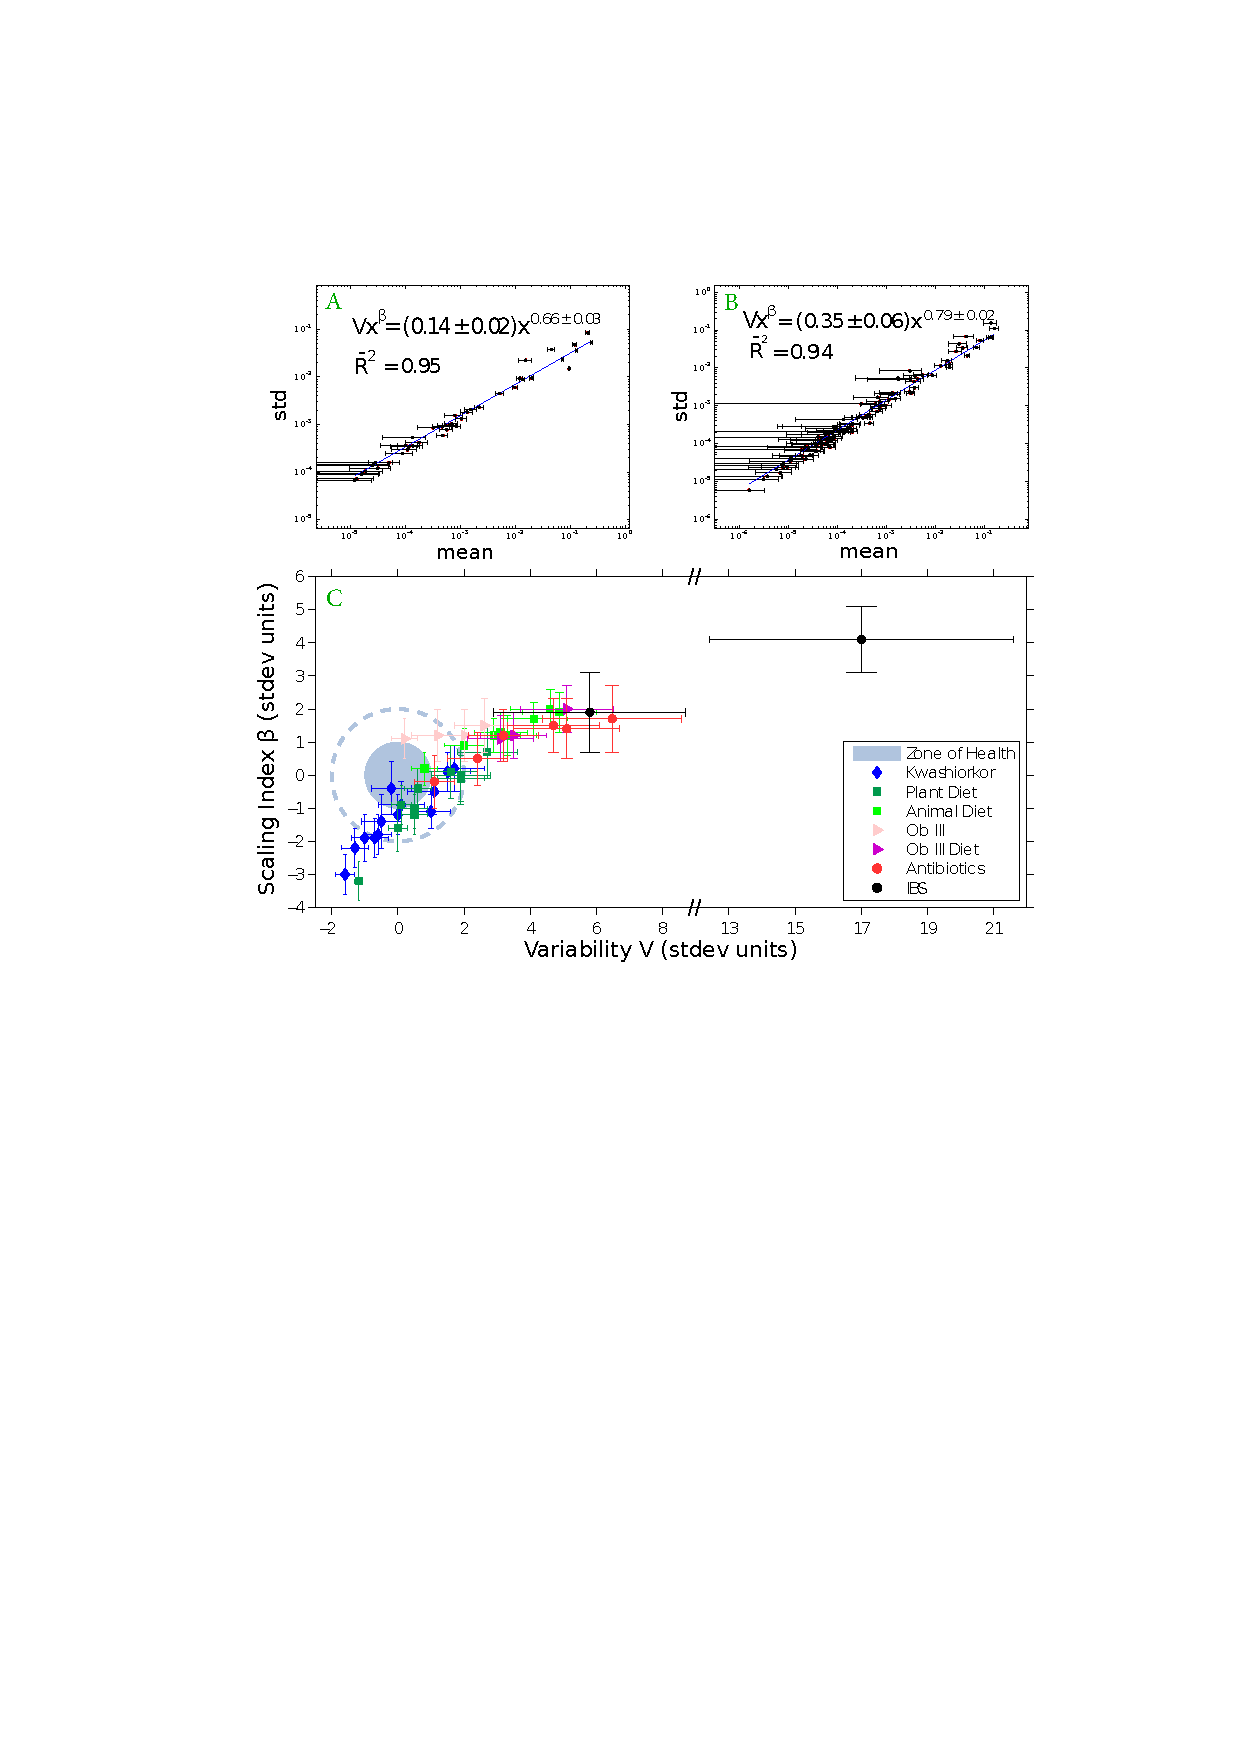
\includegraphics[width=0.9\textwidth]{results/comboplot1.pdf}
\caption{Taylor's law parameter space. X-weighted power-law fits of the standard deviations versus the mean values for each bacterial genus monitored in time. We show the fit for samples from a healthy subject (Figure A) and from a subject diagnosed with irritable bowel syndrome (Figure B) studied in our lab\cite{durban}. We have compiled all data studied in this work in Figure C. The coloured region (dashed line) corresponds to 68\% (95\%) CL region of healthy individuals in the Taylor parameter space. Points with errors place each individual gut microbiome in the Taylor space. Note that the parameters have been standardized (stdev units) to the healthy group in each study for demonstrative purposes.}
\end{figure*}

\begin{figure*}
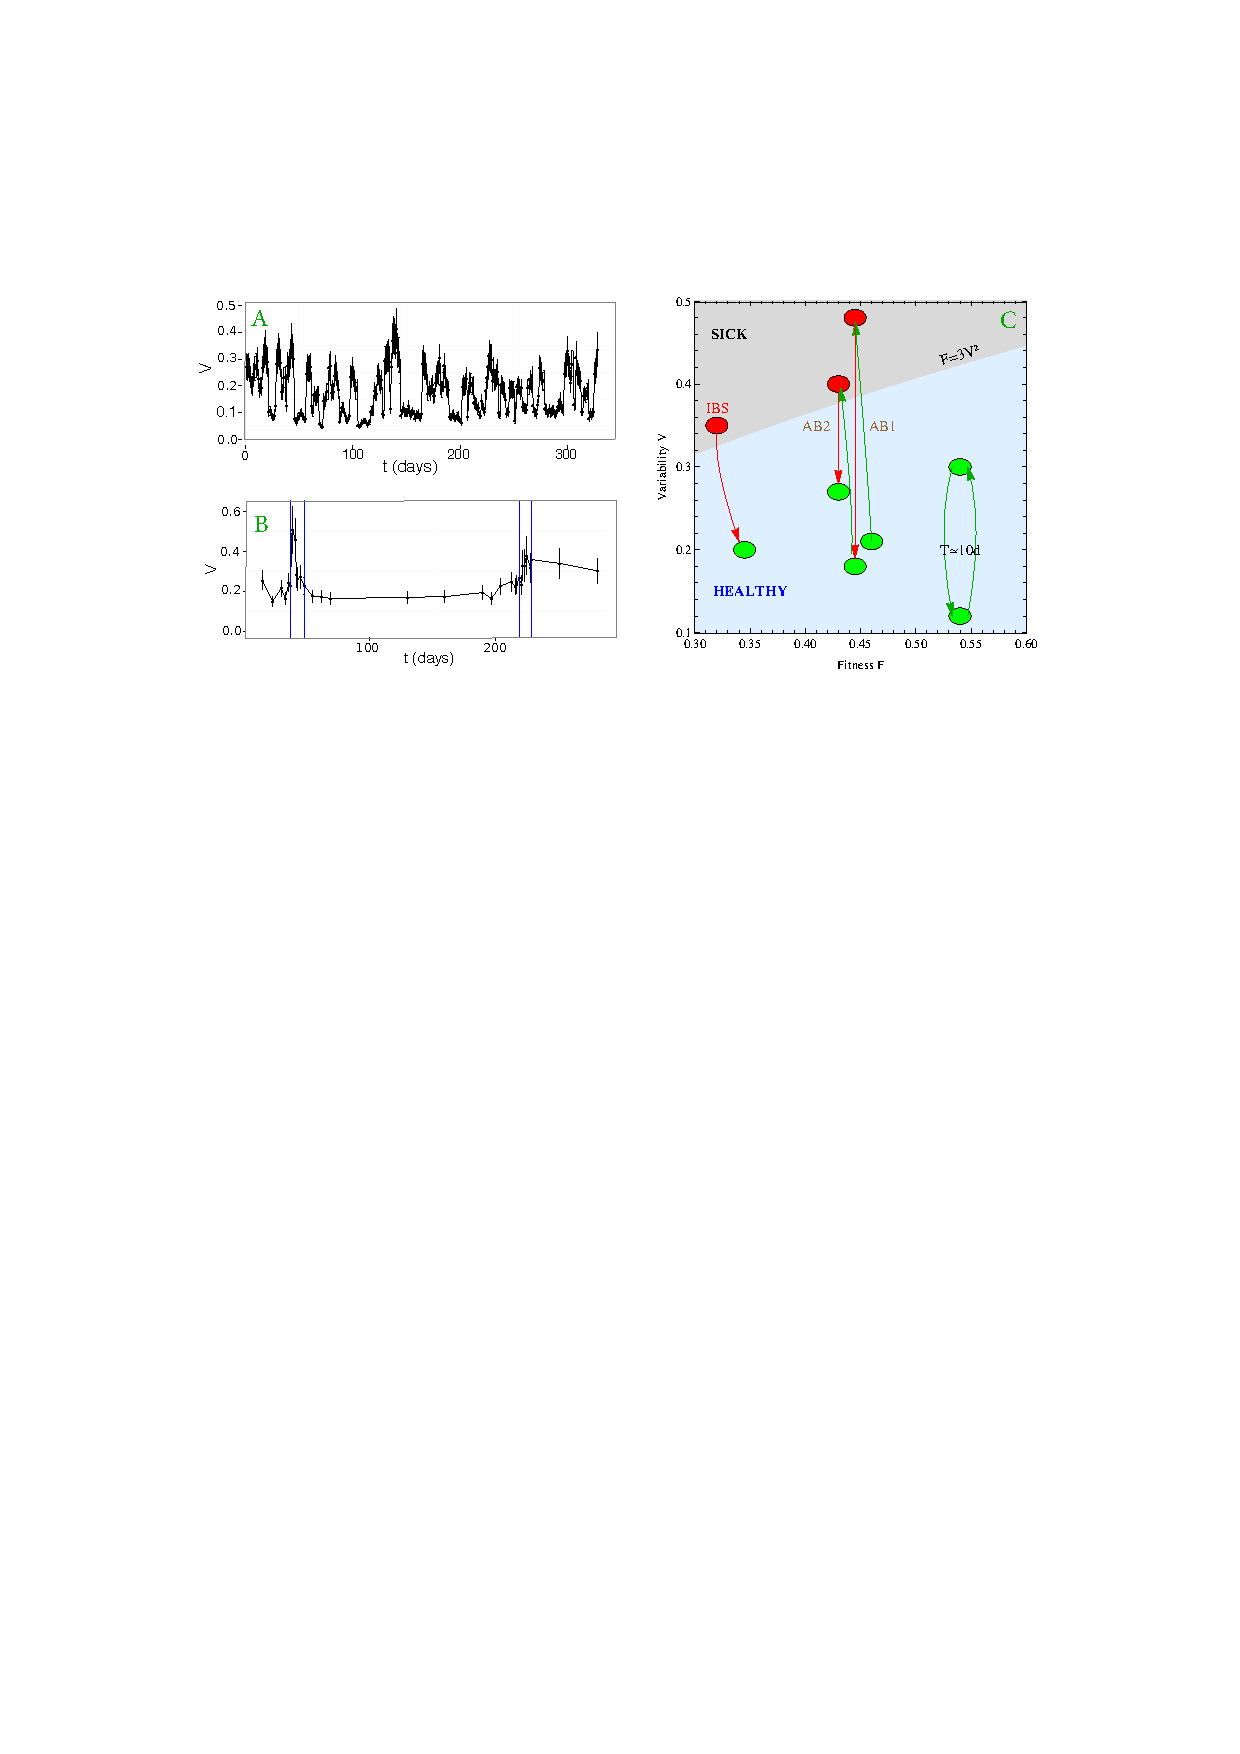
\includegraphics[width=0.9\textwidth]{results/comboplot2.pdf}
\caption{Phase space of microbiota stability. We show the Variability parameter as a function of time for the male in Caporaso's study\cite{moving} (Figure A) and for the patient D in the antibiotics study\cite{antibiotic} (Figure B). Periods of antibiotic treatment are shown by blue vertical lines. Microbiota states can be placed in the phase space F-V (Figure C). The light blue shaded region corresponds to the stable phase, while the grey shaded region is the unstable phase (the phase transition line is calculated for  $\alpha$ = $\beta$ = 0.75). We place healthy individuals (green) and individuals whose gut microbiota is threatened (antibiotics, IBS) in the phase space fitness - variability. Gut microbiota of healthy individuals over a long term span show a quasi--periodical variability (central period is ten days). We show that taking antibiotics (AB1 and AB2 correspond to first and second treatment respectively) induces a phase transition in the gut microbiota, which impacts its future changes. We also show an IBS--diagnosed patient transiting from the unstable to the stable phase.}
\end{figure*}


\subsection*{Temporal evolution of model parameters}

We have studied the time dependence of the variability $V$ and power law index $\beta$ (see Section \ref{sec:model}) by using a sliding window approach. The total number of time points are divided in subsets of five points, where next subset is defined by adding next time sampling and by eliminating the earliest one. Both parameters were calculated for each subset against the average time lapse. Figure \ref{fig:tempevo1} shows the variability  $V$ as a function of time for the largest sampling: two individuals in the Caporaso's study\cite{moving} corresponding to the gut microbiota of a male (upper plot) and a female (lower plot). Figure \ref{fig:tempevo2} shows the time evolution of $V$ for patient P2 of the IBS study\cite{IBS} (upper plot) and patient D in the antibiotics study\cite{antibiotic} (lower plot). 

\begin{figure}
	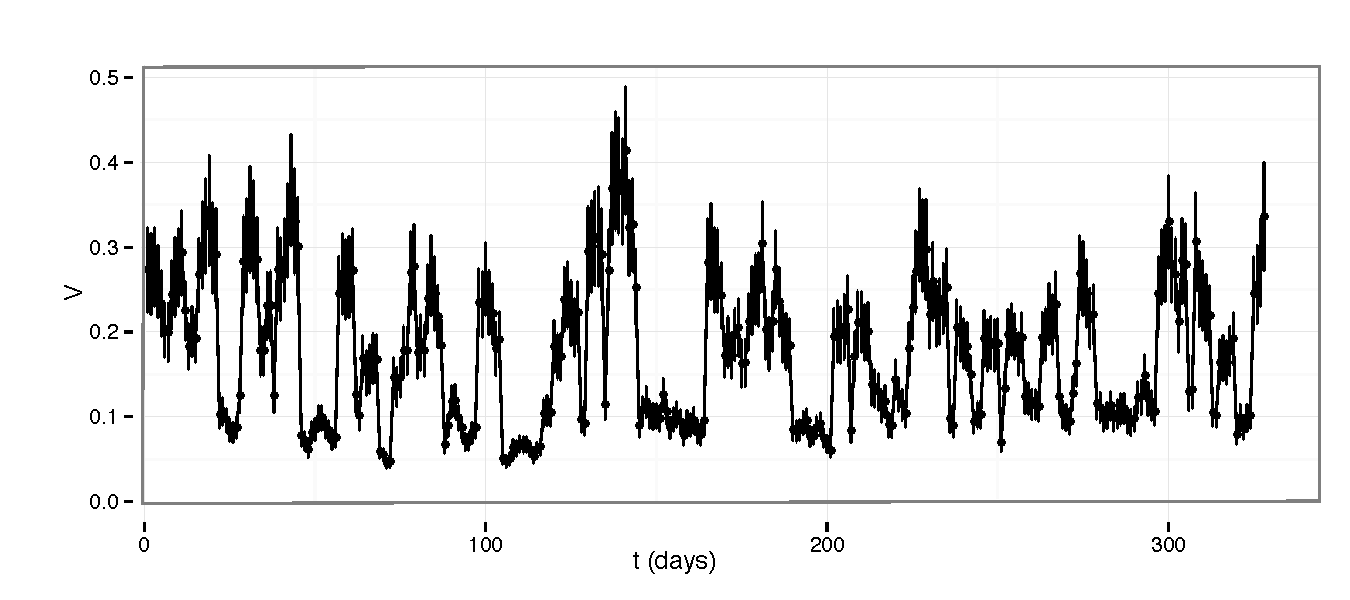
\includegraphics[width=1.0\textwidth]{results/sliwin/male_mov.pdf}
	\hspace*{3mm}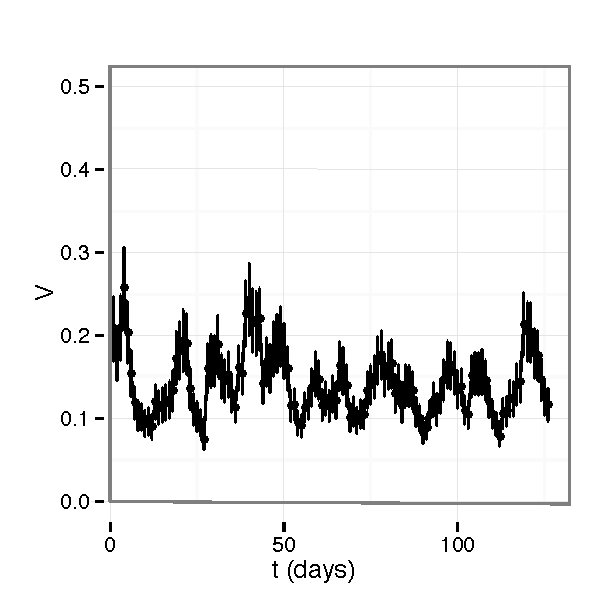
\includegraphics[width=0.448\textwidth]{results/sliwin/female_mov.pdf}
\caption{$V$ as a function of time for the two individuals in the Caporaso's study\cite{moving}: samples of gut microbiome of a male (upper plot) and a female (lower plot). Both samples show changes in the variability V with quasi--periodic behavior peaked at about 10 days. Variability grows more for the gut microbiota of the male and share a minimal value around 0.1 with the gut microbiota of the female.}
\label{fig:tempevo1}
\end{figure}

\begin{figure}
	\centering 
 	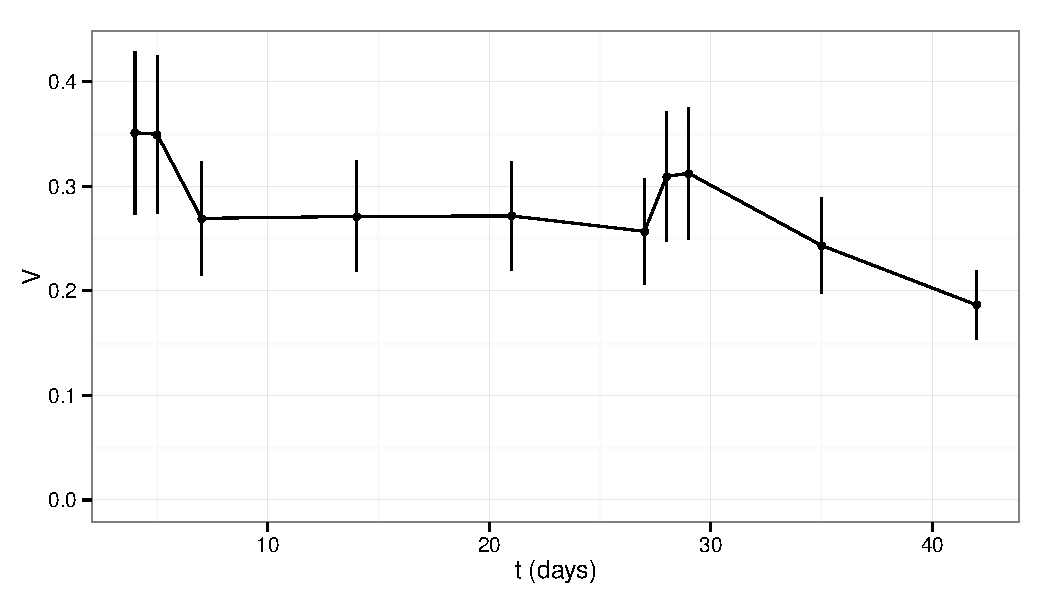
\includegraphics[width=0.8\textwidth]{results/sliwin/patP2_IBS.pdf}
  	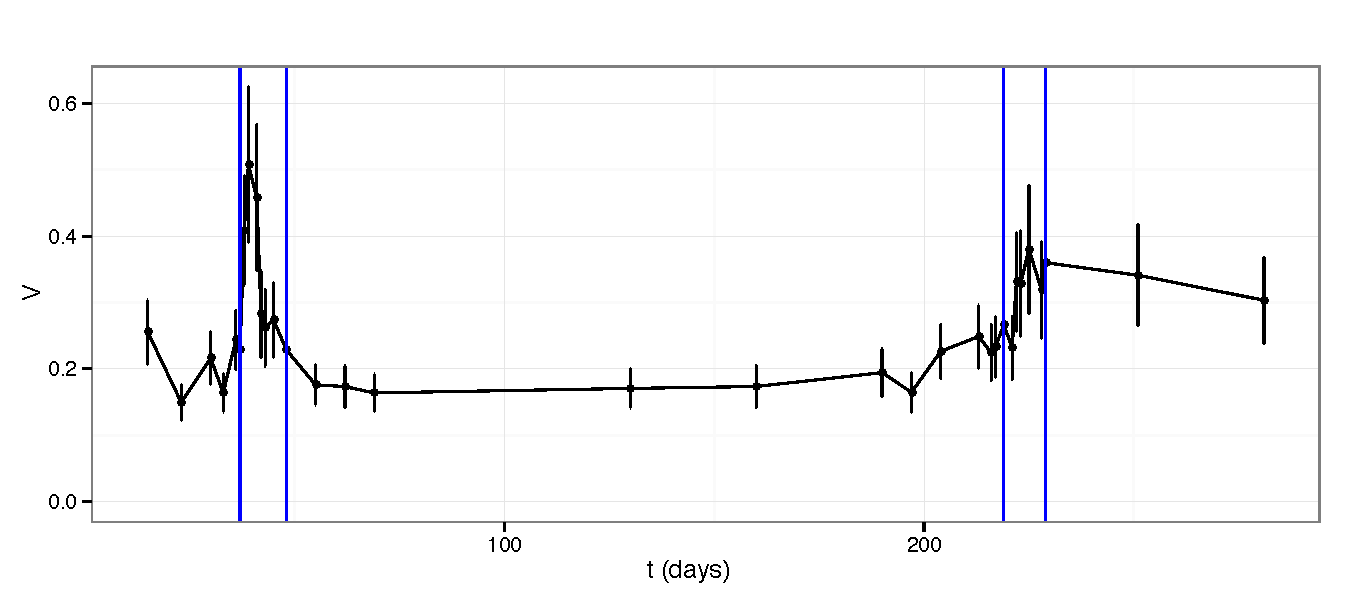
\includegraphics[width=1.0\textwidth]{results/sliwin/patD_antibio.pdf} 
\caption{$V$ as a function of time for patient P2 of the IBS study\cite{IBS} (upper plot) and patient D in the antibiotics study\cite{antibiotic} (lower plot). The variability 
of the gut microbiota of P2 decreases from above 0.3 to below 0.2, showing a slow tendency to increase the order of the system.  Antibiotic intake leaks to a quick increase of variability which lasts for a few days to recover ordering. The second antibiotic treatment shows some memory (lower increase of variability) with a slower recovery. NOTE: The blue vertical lines in the lower plot are showing the periods of antibiotic treatment.}
\label{fig:tempevo2}
\end{figure}